\documentclass[11pt]{article}

\usepackage{amsmath,amssymb,epsfig}
%\usepackage[T1]{fontenc}
%\usepackage{ae,aecompl}
\usepackage{subfigure}
\addtolength{\voffset}{-1cm}
\addtolength{\hoffset}{-1cm}
\setlength{\parindent}{0in}
\addtolength{\textwidth}{1.8cm}
\addtolength{\textheight}{1cm}
\addtolength{\parskip}{.5cm}

% Example definitions.
% --------------------
\def\e{{e^{j\omega}}}
\def\W{{W_M}}
\def\sumk{{\sum_{k=-\infty}^{\infty}}}
\def\x{{\mathbf x}}
\def\X{{\mathbf X}}
\def\Y{{\mathbf Y}}
\def\u{{\mathbf u}}
\def\U{{\mathbf U}}
\def\x{{\mathbf x}}
\def\s{{\mathbf s}}
\def\A{{\mathbf A}}
\def\y{{\mathbf y}}
\def\w{{\mathbf w}}
\def\B{{\mathbf B}}
\def\a{{\mathbf a}}
\def\D{{\mathbf D}}
\def\P{{\mathbf P}}
\def\n{{\mathbf n}}
\def\V{{\mathbf V}}
\def\R{{\mathbf R}}
\def\I{{\mathbf I}}
\def\M{{\mathbf M}}
\def\sech{{\mathrm{sech}}}
\def\L{{\cal L}}
\def\Cum{{\rm{Cum}}}
\def\var{{\rm{var}}}
\def\T{{\mathbf T}}
\def\C{{\mathbf C}}
\def\tf{{\emph{t-f}}}


% Title.
% ------
\title{\large{\textbf{EXERCISE 1}}}
\author{SGN-1156 Signal Processing Techniques\\
\texttt{http://www.cs.tut.fi/courses/SGN-1156/ex9/}\\
Department of Signal Processing\\
Tampere University of Technology}
\date{November 12, 2009}
%\author{\textbf{Assistant:}\\
%Germ{\'a}n G{\'o}mez-Herrero\\
%german.gomezherrero@tut.fi\\
%Room TE414}
%
% Author and date.
% ---------------



\begin{document}

\maketitle


\textbf{PROBLEM 1:}  Consider a system with the following input-output relationship:

\[
y[n] = \frac{1}{x[n]}+x[n-1]
\]

where $x[n]$ is the input to the system and $y[n]$ is the system's output. Is this system linear? Is it time-invariant? Is it stable?. Could you determine the ouput of the system to an arbitrary input by using only the system's impulse response?. Justify your answers. 

\vspace{1cm}

\textbf{SOLUTION:}

\textbf{Is the system linear?}

Consider the input sequence $a[n]=\alpha x_1[n]+\beta x_2[n]$ with $\alpha$ and $\beta$ being two arbitrary scalars and $x_1[n]$ and $x_2[n]$ being two arbitrary sequences. Then, if the system is linear, it must satisfy that the output to $a[n]$ is $y_a[n]=\alpha y_1[n] + \beta y_2[n]$ where $y_1[n]$ and $y_2[n]$ are the outputs of the system to the inputs $x_1[n]$ and $x_2[n]$, respectively. We can easily check that this system does not satisfy this condition and therefore the system is NOT linear:

\[
\begin{array}{lll}
y_a[n]&=&\frac{1}{\alpha\cdot x_1[n]+\beta\cdot x_2[n]}+\alpha\cdot x_1[n-1]+\beta\cdot x_2[n-1]\\ &\neq&\alpha\cdot\underbrace{\left(\frac{1}{x_1[n]}+x_1[n-1]\right)}_{y_1[n]}+\beta\cdot\underbrace{\left(\frac{1}{x_2[n]}+x_2[n-1]\right)}_{y_2[n]}
\end{array}
\]

\textbf{Is the system time-invariant?}

The system will be time invariant if a delayed input $x[n-\tau]$ produces a delayed output $y[n-\tau]$. Let us denote by $y_\tau[n]$ the output produced by $x[n-\tau]$. Then we can easily check that:

\[
y_\tau[n] = \frac{1}{x[n-\tau]}+x[n-1-\tau] =y[n-\tau]
\]

so the system is time-invariant.


\textbf{Is the system stable?}

A system is said to be BIBO stable if a bounded input signal produces necessarily a bounded output signal. Proving that a system is not stable is usually done by finding an example of a bounded input signal that produces an unbounded output. In our case, any bounded input sequence containing at least a zero will cause the output to diverge and, therefore, the system is not stable.


\textbf{Is the system's impulse response enough for determining the output of the system to an arbitrary input?}

No. It would be enough only if the system would be linear and time-invariant (LTI) but this system is not linear. 

\emph{Additional information:} The impulse response is the output of a system produced by an elementary impulse at $n=0$, i.e. by the input sequence $\delta[n]$. All discrete-time sequences can be expressed as a linear combination of impulses:

\[
\x[n] = \sum_{m=-\infty}^{\infty} x[m]\delta[n-m]
\]

and this means that knowing the response of the system to an elementary impulse at $n=0$ allows us to obtain the output by:

\[
\y[n] = \sum_{m=-\infty}^{\infty} x[m]h[n-m]
\]

that is, the output is just the linear convolution of the input sequence with the impulse response.




\vspace{1cm}



\textbf{PROBLEM 2:} Consider a system with the following input-output relationship:

\[
y[n] = (n-1)^2 x[n]
\]

where $x[n]$ is the input to the system and $y[n]$ is the system's output. Is this system linear? Is it time-invariant? Is it causal? Is it stable?

\vspace{1cm}

\textbf{SOLUTION:}

\textbf{Is the system linear?}

As we did in the first problem, we define the input sequence $a[n]=\alpha x_1[n]+\beta x_2[n]$ with $\alpha$ and $\beta$ being two arbitrary scalars and $x_1[n]$ and $x_2[n]$ being two arbitrary discrete-time signals. We will denote the output of the system to this input by $y_a[n]$. We can easily see that:


\[
\begin{array}{lll}
y_a[n] &=& (n-1)^2 \cdot\left(\alpha x_1[n]+\beta x_2[n]\right)=\\
& = & \alpha \underbrace{\left((n-1)^2 x_1[n]\right)}_{y_1[n]}+ \beta \underbrace{\left((n-1)^2 x_2[n]\right)}_{y_2[n]}
\end{array}
\]

\noindent and therefore the system is linear.



\textbf{Is the system time-invariant?}

To determine if a system is time-invariant we define a sequence $a[n]=x[n-n_0]$ where $x[n]$ is an arbitrary input sequence and $n_0$ is an arbitrary delay. If the system is time-invariant then the output produced by $a[n]$ should satisfy $y_{a}[n]=y[n-n_0]$ where $y[n]$ is the output corresponding to the input sequence $x[n]$. That is, if we shift in time the input sequence this has the effect of shifting in time the output by the same delay. 

In our case, the output obtained with a shifted input is:

\[
y_a[n] = (n-1)^2 a[n]=(n-1)^2 x[n-n_0]
\]

\noindent while the result of shifting the output of $x[n]$ is:

\[
y[n-n_0]= (n-n_0-1)^2 x[n-n_0]
\]

Clearly $y[n-n_0]\neq y_a[n]$ in general and, therefore, the system is time-variant (or shift-variant).


\textbf{Is the system causal?}

A system is causal if the output at a given time instant does not depend on future inputs. That is, the output of a causal system at time instant $n$ depends only of the inputs at time instants $n,n-1,n-2,...$. In our case we have that $y[n]$ is a function only of $x[n]$ and, therefore, the system is causal.


\textbf{Is the system stable?}

A system is said to be BIBO stable if a bounded input signal produces necessarily a bounded output signal. It is important to realize that BIBO stability requires that, for a given input (bounded) signal, the output of the system is below a fixed constant $C$ for any value of $n$. The value of the constant can be different for different input sequences but it cannot depend on the time index. 

Proving that a system is not stable is usually done by finding an example of a bounded input signal that produces an unbounded output (at least for some value of $n$). In our case, if we assume a constant input signal $x[n]=1 \;\forall n$, which is obviously bounded, then the output is:

\[
y[n] = (n+1)^2
\]

Since $|y[n]|$ grows monotonically with $n$ there is not any finite constant $C$ such that $|y[n]|<C\;\forall n$ and, therefore, the system is not stable.

Notice that the example input signal showing that a system is not stable is not always $x[n]=1 \; \forall n$. For instance in the case of PROBLEM 1 the system is not stable but the input $x[n]=1 \; \forall n$ would produce a bounded output. In the case of PROBLEM 1, the instability of the system can be made evident with any input sequence that contains at least one zero.



\textbf{PROBLEM 3:} Consider a system with the following input-output relationship:

\[
y[n] = x[n]+2x[n-5]
\]

where $x[n]$ is the input to the system and $y[n]$ is the system's output. Is this system stable?

\vspace{1cm}

\textbf{SOLUTION:}

In this case, there is not any evident input sequence that would cause the system to diverge. However, saying this is not enough to prove that the system is stable in general, i.e. to prove that $|y[n]|\leq C \; \forall n$ for any bounded input and an arbitrarily large (but finite) constant $C$. This type of proofs are most commonly done using the triangle inequality, which states that:

\[
|a+b|\leq |a| + |b|
\]

for any real numbers $a$ and $b$. We start by assuming a bounded input signal, i.e. $|x[n]|\leq K \;\forall n$ whith $K$ a constant. Then, using the triangle inequality:

\[
|y[n]| = |x[n]+2x[n-5]|\leq |x[n]| + |2x[n-5]| \leq K + 2K \qquad \forall n
\]

and, therefore, $|y[n]|\leq 3K = C \; \forall n$ which proves that the system is BIBO stable.

\textbf{PROBLEM 4 (problem 2.64 from the book):}  Determine the expression for the impulse response of the LTI system in the figure below.


\begin{figure}[h!]
	\centering
		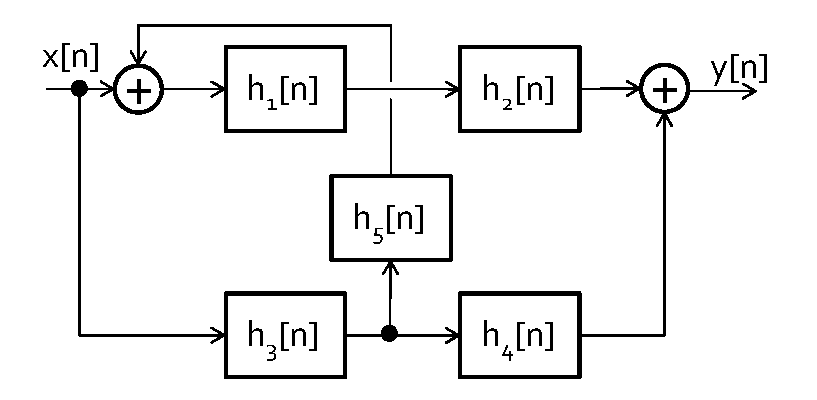
\includegraphics[width=.75\textwidth]{./system.eps}
	%\caption{dagd}
	%\label{fig:system}
\end{figure}

\vspace{1cm}

\textbf{SOLUTION:}


The first thing that you should try to do in this type of problems is to simplify as much as possible the system diagram by putting together sub-systems like $h_1[n]$ and $h_2[n]$ which do not have any connection coming or leaving from between them. Those two systems a single single system with impulse reponse $h_1[n]\ast h_2[n]$. Moreover, we should name any intermediate connection of the diagram to simplify the operations below:

\begin{figure}[h!]
	\centering
		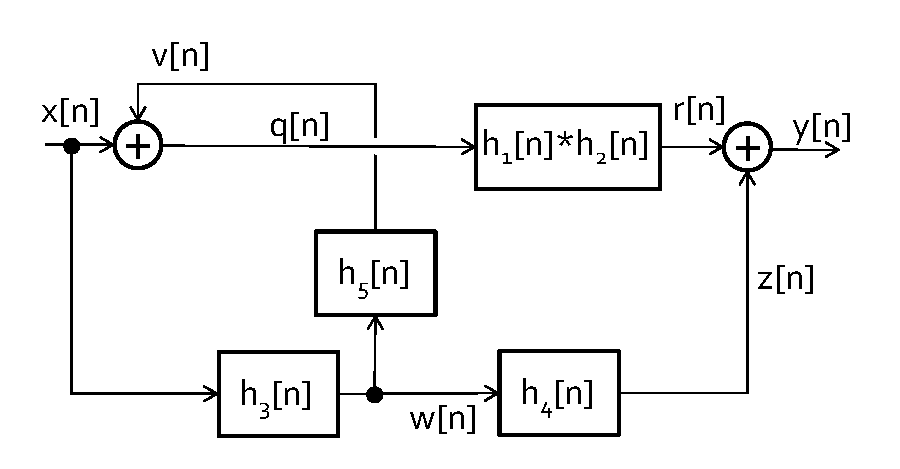
\includegraphics[width=.75\textwidth]{./system2.eps}
	%\caption{dagd}
	%\label{fig:system}
\end{figure}


From the diagram above we can see that we have 7 unknowns: $y[n]$, $r[n]$, $z[n]$, $w[n]$, $v[n]$, $q[n]$ and $x[n]$. Since we want to solve the system up to the point that $y[n]$ is written in terms of $x[n]$ this means that we need to write 6 equations to find the solution:

\begin{eqnarray}
y &=& r+z\\
r &=& h_1\ast h_2 \ast q\\
z &=& h_4\ast w\\
v &=& h_5\ast w\\
w &=& h_3 \ast x\\
q &=& v+x
\end{eqnarray}

Combining all the equations above we easily reach the result:

\[
y = \left(h_1\ast h_2 \ast h_3\ast h_5+h_1\ast h_2+h_3\ast h_4\right)\ast x
\]

And the overall impulse response of the system is:

\[
h[n]=h_1[n]\ast h_2[n] \ast h_3[n]\ast h_5[n]+h_1[n]\ast h_2[n]+h_3[n]\ast h_4[n]
\]


\vspace{1cm}

\textbf{PROBLEM 5 (problem 2.48 from the book):} A periodic sequence $\tilde{x}[n]$ with a period $N$ is applied as an input to an LTI discrete-time system characterized by an impulse response $h[n]$ generating an output $y[n]$. Is $y[n]$ a periodic sequence? If it is, what is its period?

\vspace{1cm}

\textbf{SOLUTION:}

$\tilde{x}[n]$ is periodic $\Longleftrightarrow\hat{x}[n]=\hat{x}[n+kN]$, where $k\in\mathbb{Z}$.

The output of the system to this periodic input will be:

\[
y[n] = \sum_{m=-\infty}^{\infty}h[m]\tilde{x}[n-m]
\]

and we can check that indeed $y[n]$ is periodic since $y[n+kN]=y[n]\;\forall k \in\mathbb{Z}$:

\[
y[n+kN] = \sum_{m=-\infty}^{\infty}h[m]\tilde{x}[n+kN-m]=\sum_{m=-\infty}^{\infty}h[m]\tilde{x}[n-m]=y[n]
\]


\vspace{1cm}

\textbf{PROBLEM 6 (problem 2.36 from the book):} For each of the following systems, where $y[n]$ and $x[n]$ are, respectively, the output and input sequences, determine whether the system is (1) linear, (2) causal, (3) stable, (4) shift-invariant.


\begin{itemize}
\item[(a)] $y[n]=n^3x[n]$

\item[(b)] $y[n]=(x[n])^5$


\item[(c)] $y[n]=\beta+\sum_{l=0}^{3} x[n-l] \quad \beta=\textrm{constant}$.

\item[(d)] $y[n]=\ln(2+|x[n]|)$ 


\item[(e)] $y[n]=\alpha x[-n+2]$

\item[(f)] $y[n]=x[n-4]$


\end{itemize}



\vspace{1cm}

\textbf{SOLUTION:}

\textbf{(a)} $y[n]=n^3x[n]$

In the same way as in problems 1 and 2 we can easily find that this sytem is linear, causal, unstable and time-variant.

\textbf{(b)} $y[n]=(x[n])^5$

The system is nonlinear, noncausal, stable and time-invariant. 

\textbf{(c)} $y[n]=\beta+\sum_{l=0}^{3} x[n-l] \quad \beta=\textrm{constant}$.

The system is nonlinear, causal, stable, and time-invariant. Notice that constant $\beta$ is making the system nonlinear.

\textbf{(d)} $y[n]=\ln(2+|x[n]|)$ 

The system is nonlinear, causal, stable, and time-invariant.


\textbf{(e)} $y[n]=\alpha x[-n+2]$

The system is obviously linear. Notice however that it is not causal in general since for any time instant $n<1$ the output depends on future inputs. The system is stable. 


The system is time-variant. If we consider an input sequence $x_{\tau}[n]=x[n-\tau]$ then the output will be:

\[
y_{\tau}[n] = \alpha x_{\tau}[-n+2] = \alpha x[-n+2-\tau]
\]

However,

\[
y[n-\tau] = \alpha x[-(n-\tau)+2]=\alpha x[-n+\tau+2]\neq y_{\tau}[n]
\]

and, therefore, the system is time-variant.

\textbf{(f)} $y[n]=x[n-4]$

This system is linear, causal, stable and time-invariant.

\end{document}